\documentclass[aspectratio=169, xetex, 12pt]{beamer}  % 16:9宽屏，指定xelatex编译

% ==================== 主题与外观设置 ====================
\usetheme{Madrid}
\usecolortheme{default}
\useoutertheme{infolines}  % 页眉显示导航信息
\setbeamertemplate{navigation symbols}{}   % 去除导航符号
\setbeamertemplate{blocks}[rounded][shadow=true]  % 圆阴影块

% 自定义颜色（微调，使定理环境更舒适）
\definecolor{myblue}{RGB}{0,82,155}
\setbeamercolor{block title}{fg=white,bg=myblue}
\setbeamercolor{block body}{fg=black,bg=blue!5}

% ==================== 英文 & 数字 设置为 Times New Roman ====================
\usepackage{fontspec}
\setmainfont{Times New Roman}       % 英文正文
\setsansfont{Times New Roman}       % 无衬线英文（beamer默认）
\setmonofont{Times New Roman}      % 等宽英文/数字

% ==================== 中文支持 ====================
\usepackage[UTF8, scheme=plain]{ctex}  % scheme=plain避免修改章节格式
\setCJKmainfont{SimHei}   % 使用黑体作为主要中文字体
\setCJKsansfont{SimHei}
\setCJKmonofont{SimHei}

% ==================== 数学与符号 ====================
\usepackage{amsmath, amssymb}  % 数学宏包
\usepackage{bm}            % 粗体数学符号
\usepackage{newtxmath}     % Times风格数学字体（必须保留）

% ==================== 图表与表格 ====================
\usepackage{graphicx}
\usepackage{subcaption}    % 并排子图
\usepackage{booktabs}      % 三线表
\usepackage{siunitx}       % 数值对齐

% ==================== 其他工具 ====================
\usepackage{hyperref}      % 超链接
\usepackage{caption}       % 定制标题
\captionsetup{labelformat=empty, justification=centering}

% ==================== 定理环境重定义 ====================
\newtheorem{defn}{定义}[section]
\newtheorem{thm}{定理}[section]
\newtheorem{lem}{引理}[section]
\newtheorem{prop}{命题}[section]
\newtheorem{cor}{推论}[section]

\setbeamercolor{block title theorem}{fg=white,bg=myblue}
\setbeamercolor{block body theorem}{fg=black,bg=blue!5}
\setbeamertemplate{theorem begin}{%
	\begin{block}{\inserttheoremname \inserttheoremnumber}
	}
	\setbeamertemplate{theorem end}{\end{block}}

\setbeamercolor{block title definition}{fg=white,bg=myblue!70!black}
\setbeamertemplate{definition begin}{%
	\begin{block}{\inserttheoremname \inserttheoremnumber}
	}
	\setbeamertemplate{definition end}{\end{block}}

% ==================== 标题页信息 ====================
\title{利用有限元方法数值求解热传导方程}
\author[张雨]{报告人：张雨\\ \vspace{0.2cm} 指导教师：刘鸿雁 \quad 讲师}
\institute{贵州大学\\数学与统计学院}
\date{2026年5月22日}
\begin{document}
	
	% ---------- 封面 ----------
	\begin{frame}
		\titlepage
	\end{frame}
	
	% ---------- 目录 ----------
	\begin{frame}{目录}
		\tableofcontents
	\end{frame}
	
	\section{研究背景与意义}
	
\begin{frame}{研究背景}
\[
\left\{
\begin{aligned}
	\frac{\partial u}{\partial t} - \alpha \Delta u &= f(\boldsymbol{x},t), && (\boldsymbol{x},t) \in \Omega \times (0,T], \\
	u(\boldsymbol{x},0) &= u_0(\boldsymbol{x}), && \boldsymbol{x} \in \Omega, \\
	u(\boldsymbol{x},t) &= g(\boldsymbol{x},t), && (\boldsymbol{x},t) \in \partial\Omega \times (0,T].
\end{aligned}
\right.
\]
	\begin{itemize}
		\setlength{\itemsep}{0.7em}   % 外层项间距
		\item 热传导方程是二阶线性抛物型偏微分方程，描述热量在介质中的扩散过程。
		\item 广泛应用于工程传热分析、地热模拟、材料热处理等领域且应用已从传统传热分析拓展到诸多新兴领域。
		\item 面对复杂几何形状、多变材料属性和复杂边界条件时，解析解难以获得甚至不存在。
			\vspace{0.3em}
		\item 研究定位：本文探究利用分片线性有限元方法求解热传导方程。
	\end{itemize}
\end{frame}

\begin{frame}{研究意义}
	\begin{enumerate}
		\setlength{\itemsep}{0.7em}   % 与外层一致
		\item \textbf{理论意义：}
		\begin{itemize}
			\setlength{\itemsep}{0.4em}   % 内层略紧凑，但仍比默认宽
			\item 对一维热传导方程的空间半离散格式及全离散 BDF2-P1 格式的稳定性分析与误差估计，深化对偏微分方程数值解法的理论认识。
			\item 理论框架可推广至一般抛物型方程。
		\end{itemize}
		\vspace{0.3em}
		\item \textbf{实际意义：}
		\begin{itemize}
			\setlength{\itemsep}{0.4em}
			\item 为工程热分析、材料科学、环境模拟提供精确仿真工具。
			\item 推广二维模型及FreeFem++ 实现，降低数值模拟的技术门槛。
		\end{itemize}
			\vspace{0.3em}
		\item \textbf{研究目标：}
		发展具有普适性的数值解法理论。
\end{enumerate}
\end{frame}
	
	\section{预备知识}
	
\begin{frame}{预备知识}
	\begin{itemize}
		\item \textbf{Sobolev 空间 $H^{\,m}(\Omega)$}
		\[
		H^{\,m}(\Omega) = \{ u \in L^2(\Omega) : D^\alpha u \in L^2(\Omega), \text{ 对所有 } |\alpha| \le m \}.
		\]
		特别地，$H^{\,m}_0(\Omega)$ 为边界上为零的 $H^{\,m}(\Omega)$ 子空间。
		\vspace{2em}
		\item \textbf{分片线性有限元空间 (P1)：}
		设 $\mathcal{T}_h$ 为 $\Omega$ 的剖分，定义有限元空间：
		\[
		V_h = \{ v_h \in C(\overline{\Omega}) : v_h|_K \in \mathrm{P}1(K), \forall K \in \mathcal{T}_h\}.
		\]
	\end{itemize}
\end{frame}
\begin{frame}{预备知识}
	\begin{itemize}
		\item \textbf{椭圆投影 $P_h: H^1_0(\Omega) \to V_h$：}
		\[
		a(P_h u, v) = a(u, v), \quad \forall v \in V_h,
		\]
		其中 $a(u,v) = \int_{\Omega} \nabla u \cdot \nabla v \,dx$。
			\vspace{2em}
		\item \textbf{Poincaré 不等式：}
		如果 $\Omega$ 为连通且在一个方向上有界的区域，则对每个非负整数 $m \in \mathbb{N}$，存在 $C_p=\text{const} > 0$，使得
		\[
		\|v\|_{m,\Omega} \leq C_p |v|_{m,\Omega}, \quad \forall v \in H_0^{\,m}(\Omega).
		\]
	\end{itemize}
\end{frame}
\begin{frame}{模型问题}
	\begin{itemize}
		\item 	考虑带Dirichlet边界条件的一维热传导问题：
		\[
		\begin{cases}
			\dfrac{\partial u}{\partial t} - \alpha u_{xx} = f(x,t), & (x,t) \in \Omega \times (0,T], \\[4pt]
			u(x,t) = 0, & (x,t) \in \partial\Omega \times (0,T], \\[4pt]
			u(x,0) = u_0(x), & x \in \Omega.
		\end{cases}
		\]
	\end{itemize}

\end{frame}
	
	\begin{frame}{变分形式}
		\begin{itemize}
			\item 	定义双线性形式：
			\[
			a(u,v) = \int_{\Omega} \nabla u \cdot \nabla v \,dx.
			\]
		

		变分形式：求 \( u(t) \in H^1_0(\Omega) \)，使得对任意 \( v \in H^1_0(\Omega) \) 有
		\[
		\left( \frac{\partial u}{\partial t}, v \right) + a(u,v) = (\,f, v), \quad t \in (0,T],
		\]
		其中 \( (\cdot,\cdot) \) 为 \( L^2(\Omega) \) 内积。
	\end{itemize}
	\end{frame}
	
	\section{空间半离散和全离散BDF2-P1格式}
	
	\begin{frame}{半离散格式-空间剖分}
		\begin{itemize}
			\item 对空间变量采用分片线性有限元离散\\
		\vspace{1em}
			将求解区间 $\Omega = [a,b]$ 剖分为 $N$ 个子区间，节点为
			\[
			a = x_1 < x_2 < \cdots < x_{N+1} = b.
			\]
	\vspace{1em}
	\item \textbf{有限元空间 $V_h \subset H_0^1(\Omega)$}
			\[
			V_h = \left\{v_h \in C(\overline{\Omega}) : \left. v_h \right|_{[x_{i-1},x_i]} \in \mathrm{P}1, \ i = 2, \ldots, N+1,\ v_h(a) = v_h(b) = 0 \right\}.
			\]
		
		其中 $\mathrm{P}1$ 表示一次多项式。
	\end{itemize}
	\end{frame}
	
\begin{frame}{基函数}
   \begin{itemize}
   	\setlength{\itemsep}{0.7em}  
   	\item 有限元空间 $V_h$ 由基函数 $\{\phi_i(x)\}$ 张成
   	\item 基函数 $\phi_i(x)$ 满足 $\phi_i(x_j) = \delta_{ij}$
\[	\phi_i(x) =
\begin{cases}
	\dfrac{x - x_{i-1}}{h}, & x \in [x_{i-1}, x_i], \\[6pt]
	\dfrac{x_{i+1} - x}{h}, & x \in [x_i, x_{i+1}], \\
	0, & \text{其他},
\end{cases}
\qquad i = 2, \dots, N-1.\]
		\item 边界基函数
		
		\[
		\phi_1(x) =
		\begin{cases}
			\dfrac{x_2-x}{h}, & x \in [x_1, x_2], \\
			0, & \text{其他},
		\end{cases}
		\quad
		\phi_{N+1}(x) =
		\begin{cases}
			\dfrac{x-x_N}{h}, & x \in [x_N, x_{N+1}], \\
			0, & \text{其他}.
		\end{cases}
		\]

\end{itemize}
\end{frame}

\begin{frame}{基函数图像}
	\begin{figure}
		\centering
		\includegraphics[width=0.5\linewidth]{jihanshu.png}
		\caption{线性插值基函数示意图}
		\label{fig:basis-functions}
	\end{figure}
\end{frame}
	\begin{frame}{半离散格式—方程与解的形式}
		\begin{itemize}
			\setlength{\itemsep}{0.7em} 
			\item 寻找 $u_h(\cdot,t) \in V_h$，使得对任意试验函数 $v \in V_h$ 满足
			\[
			\begin{cases}
				\Bigl( \dfrac{\partial u_h}{\partial t}, v \Bigr) + a(u_h,v) = (\, f,v), & \forall v \in V_h, \\[6pt]
				u_h(x,0) = u_{0,h}(x), & x \in \Omega.
			\end{cases}
			\]
		\item 有限元解可表示为基函数的线性组合形式：
		\[
		u_h(x,t) = \sum_{j=2}^{N} u_j(t) \phi_j(x),
		\]
		其中 $u_j(t) = u_h(x_j,t)$。
			\end{itemize}
	\end{frame}
	
	\begin{frame}{矩阵向量形式}
		将 $u_h(x,t)$代入半离散变分格式，并取测试函数$v=\phi_i$可得：
	\[	
	\sum_{j=2}^N \dot{u}_j(t)(\phi_j, \phi_i) + \sum_{j=2}^N u_j(t)(\nabla \phi_j, \nabla \phi_i) = (\, f, \phi_i), \quad i = 2, \dots, N,
	\]
		其中$\dot{u}_j(t)=\frac{d{u}_j(t)}{dt}$。半离散矩阵形式：
		\[	M\dot{\mathbf{u}}(t) + A\mathbf{u}(t) = F,\]
		其中 $M$ 为质量矩阵，$A$ 为刚度矩阵，$F$ 为载荷向量，$\mathbf{u}(t) = [u_1(t), \dots, u_N(t)]^\top$。
		\begin{itemize}
			\item $M_{ij} = (\phi_j, \phi_i) = \int_a^b \phi_j \phi_i \,dx,$
			\item $A_{ij} = a(\phi_j, \phi_i) = \int_a^b \nabla \phi_j \cdot \nabla \phi_i \,dx,$
			\item $F_i = (\, f^{\;m}, \phi_i) = \int_a^b f(x,t_m) \phi_i \,dx.$
		\end{itemize}
	\end{frame}
	\begin{frame}{全离散BDF2-P1格式}
			\begin{itemize}
		\item 二阶向后差分格式（BDF2）：
		\[
		\frac{\partial u}{\partial t} \bigg|_{t=t_m} \approx \frac{3u^m - 4u^{m-1} + u^{m-2}}{2\Delta t},
		\]
		其中 $t_m=m\Delta t,\ m=0,1,\dots$。
\item BDF2-P1全离散格式
			\[
			\begin{cases}
				\left( \dfrac{3u_h^m - 4u_h^{m-1} + u_h^{m-2}}{2\tau}, v\right) + a(u_h^m, v) = (\, f^{\;m}, v), \quad \forall v \in V_h, \\[8pt]
				u_h^0 = u_{0,h}, \quad u_h^1 \text{ 由向后欧拉法求解得到},
			\end{cases}
			\]
			其中 $u_h^m \approx u_h(x,t_m)$，$f^{\;m} = f(x, t_m)$，记时间步长 $\Delta t=\tau$。
			\item	全离散矩阵形式
			\[	\left( \frac{3}{2\tau} M + A\right) \mathbf{u}^m
			= M \left( \frac{4}{2\tau} \mathbf{u}^{m-1} - \frac{1}{2\tau} \mathbf{u}^{m-2} \right) + F.\]
	
		\end{itemize}
	\end{frame}
	\begin{frame}{稳定性分析}
		\begin{thm}[全离散 BDF2-P1 格式的稳定性]
			设 $u_h^m$ 是全离散格式的解，源项 $f \in L^\infty(0,T; L^2(\Omega))$。则存在与 $\tau, h$ 无关的常数 $C > 0$，使得对任意 $m \geq 2$，以下稳定性估计成立：
			\[
			\| u_h^M \| + \tau \sum_{k=2}^m \| \nabla u_h^k \| 
			\leq C \left( \| u_h^0 \| + \| u_h^1 \| + \tau \sum_{k=2}^m \| \,f^{\;k} \| \right),
			\]
			其中 $\|\cdot\|$ 表示 $L^2(\Omega)$ 范数。
		\end{thm}
	\end{frame}
	
	\begin{frame}{误差估计}
		\begin{thm}[全离散 BDF2-P1 格式的误差估计]
			设 $u(x,t_m)$ 和 $u_h^m$ 分别是原问题的解析解与全离散解。则满足如下误差估计：
			\[
			\max_{2 \le m \le M} \|u(t_m) - u_h^m\| \le C (\tau^2 + h^{k+1}) \|u\|_{C^3([0,T];H^{k+1})},
			\]
			其中常数 $C > 0$ 依赖于终时 $T$，但与 $\tau, h$ 无关。对于 $P1$ 元，$k=1$，空间收敛阶为 $O(h^2)$。
		\end{thm}
		
	\end{frame}
	
	\section{数值实验}
	
\begin{frame}{一维数值算例}
	\begin{itemize}
		\item \textbf{例1.} 考虑一维非齐次热传导方程初边值问题：
		\[
		\begin{cases}
			u_t - \alpha\,u_{xx} = G\sin(\pi x), & x\in(0,1),\; t\in(0,1),\\[3pt]
			u(0,t) = 0,\; u(1,t) = 0, & t\in[0,1],\\[3pt]
			u(x,0) = 0, & x\in[0,1].
		\end{cases}
		\]
		取参数 $\alpha=1,\ G=2$，解析解为
		\[
		u(x,t)=\dfrac{2}{\pi^2}\bigl(1-\mathrm{e}^{-\pi^2 t}\bigr)\sin(\pi x).
		\]
	\end{itemize}

\end{frame}
	
	\begin{frame}{一维数值算例-数值结果验证}
		\begin{center}
			\includegraphics[width=0.6\textwidth]{shili-one.png} \\
			\vspace{0.2cm}
			\small 图1：数值解与解析解在 $T=1$ 时刻的对比曲线
		\end{center}
		
	\end{frame}
	
	\begin{frame}{一维数值算例-数值结果验证 }
		\begin{center}
			\begin{minipage}[b]{0.44\textwidth}
				\centering
				\includegraphics[width=\linewidth]{jiexijie.png}
				\small (a) 解析解三维演化曲面
			\end{minipage}
			\hfill
			\begin{minipage}[b]{0.44\textwidth}
				\centering
				\includegraphics[width=\linewidth]{shuzhijie.png}
				\small (b) 数值解三维演化曲面
			\end{minipage}
		\end{center}
		\vspace{0.2cm}
		\begin{center}
			\small\bfseries 图2：解析解与BDF2-P1数值解的三维演化过程对比
		\end{center}
	\end{frame}
	
	\begin{frame}{一维数值算例-收敛性分析}
		\begin{columns}[T, onlytextwidth]
			\begin{column}{0.48\textwidth}
				\centering
				\small
				\textbf{空间收敛性（$\tau=0.001$ 固定）}
				\vspace{0.1cm}
				\begin{tabular}{cccc}
					\toprule
					$N_x$ & $h$ & $\|u-u_h\|_{L^2}$ & 阶 \\
					\midrule
					10 & 0.10000 & $1.556\times10^{-6}$ & -- \\
					20 & 0.05000 & $2.115\times10^{-7}$ & 2.88 \\
					40 & 0.02500 & $4.314\times10^{-8}$ & 2.29 \\
					60 & 0.01667 & $1.929\times10^{-8}$ & 1.99 \\
					80 & 0.01250 & $1.148\times10^{-8}$ & 1.80 \\
					\bottomrule
				\end{tabular}
			\end{column}
			\begin{column}{0.48\textwidth}
				\centering
				\small
				\textbf{时间收敛性（$h=0.005$ 固定）}
				\vspace{0.1cm}
				\begin{tabular}{cccc}
					\toprule
					$N_t$ & $\tau$ & $\|u-u_h\|_{L^2}$ & 阶 \\
					\midrule
					16  & 0.06250 & $9.593\times10^{-6}$ & -- \\
					32  & 0.03125 & $2.187\times10^{-6}$ & 2.13 \\
					64  & 0.01562 & $5.013\times10^{-7}$ & 2.13 \\
					128 & 0.00781 & $1.200\times10^{-7}$ & 2.06 \\
					256 & 0.00391 & $3.032\times10^{-8}$ & 1.99 \\
					\bottomrule
				\end{tabular}
			\end{column}
		\end{columns}
	\end{frame}
	
\begin{frame}{二维情形}
	\begin{itemize}
		\item \textbf{例2.}二维热传导方程初边值问题：
		\[
		\begin{cases}
			\dfrac{\partial u}{\partial t} - \alpha \Delta u =e^{-t}\sin(\pi x)\sin(\pi y), & (x, y)\in\Omega,\; t\in(0,T], \\[6pt]
			u(x, y, 0) =0, & (x, y)\in\Omega, \\[6pt]
			u(x, y, t) = 0, & (x, y)\in\partial\Omega,\; t>0.
		\end{cases}
		\]
		取参数 $\Omega = [0,1]^2$, $\alpha = 1.0$, $T=1.0$，解析解为
		\[
		u(x,y,t) = \frac{1}{2\pi^2-1}\bigl(e^{-t}-e^{-2\pi^2 t}\bigr)\sin(\pi x)\sin(\pi y)
		\]
	\end{itemize}
	
\end{frame}
	
	\begin{frame}{二维情形-数值结果}
		\begin{center}
			\begin{minipage}[b]{0.45\textwidth}
				\centering
				\includegraphics[width=\linewidth]{exact_solution.eps}
				\footnotesize  图3：终止时刻解析解
			\end{minipage}
			\hfill
			\begin{minipage}[b]{0.45\textwidth}
				\centering
				\includegraphics[width=\linewidth]{numerical_solution.eps}
				\footnotesize  图4：终止时刻数值解
			\end{minipage}
		\end{center}
		
	\end{frame}
	
\begin{frame}{非线性算例}
	\begin{itemize}
		\item \textbf{例3.}非线性抛物型方程初边值问题：
		\begin{equation}\label{eq:nonlinear}
			\begin{cases}
				\dfrac{\partial u}{\partial t} + u \dfrac{\partial u}{\partial x}- \nu \dfrac{\partial^2 u}{\partial x^2}=0, & (x, t) \in (0, 1) \times (0, 1], \\
				u(0, t) = 0, \quad u(1, t) = 0, & t \in [0, 1], \\
				u(x, 0) = \sin(\pi x), &x \in [0, 1],
			\end{cases}
		\end{equation}
		其中粘性系数 $\nu=0.1$。解析解由第一类修正 Bessel 函数的无穷级数给出。
	\end{itemize}

\end{frame}
	
	\begin{frame}{非线性算例-数值结果}
		\vspace{-0.2cm}
		\begin{columns}[T, onlytextwidth]
			\begin{column}{0.40\textwidth}
				\centering
				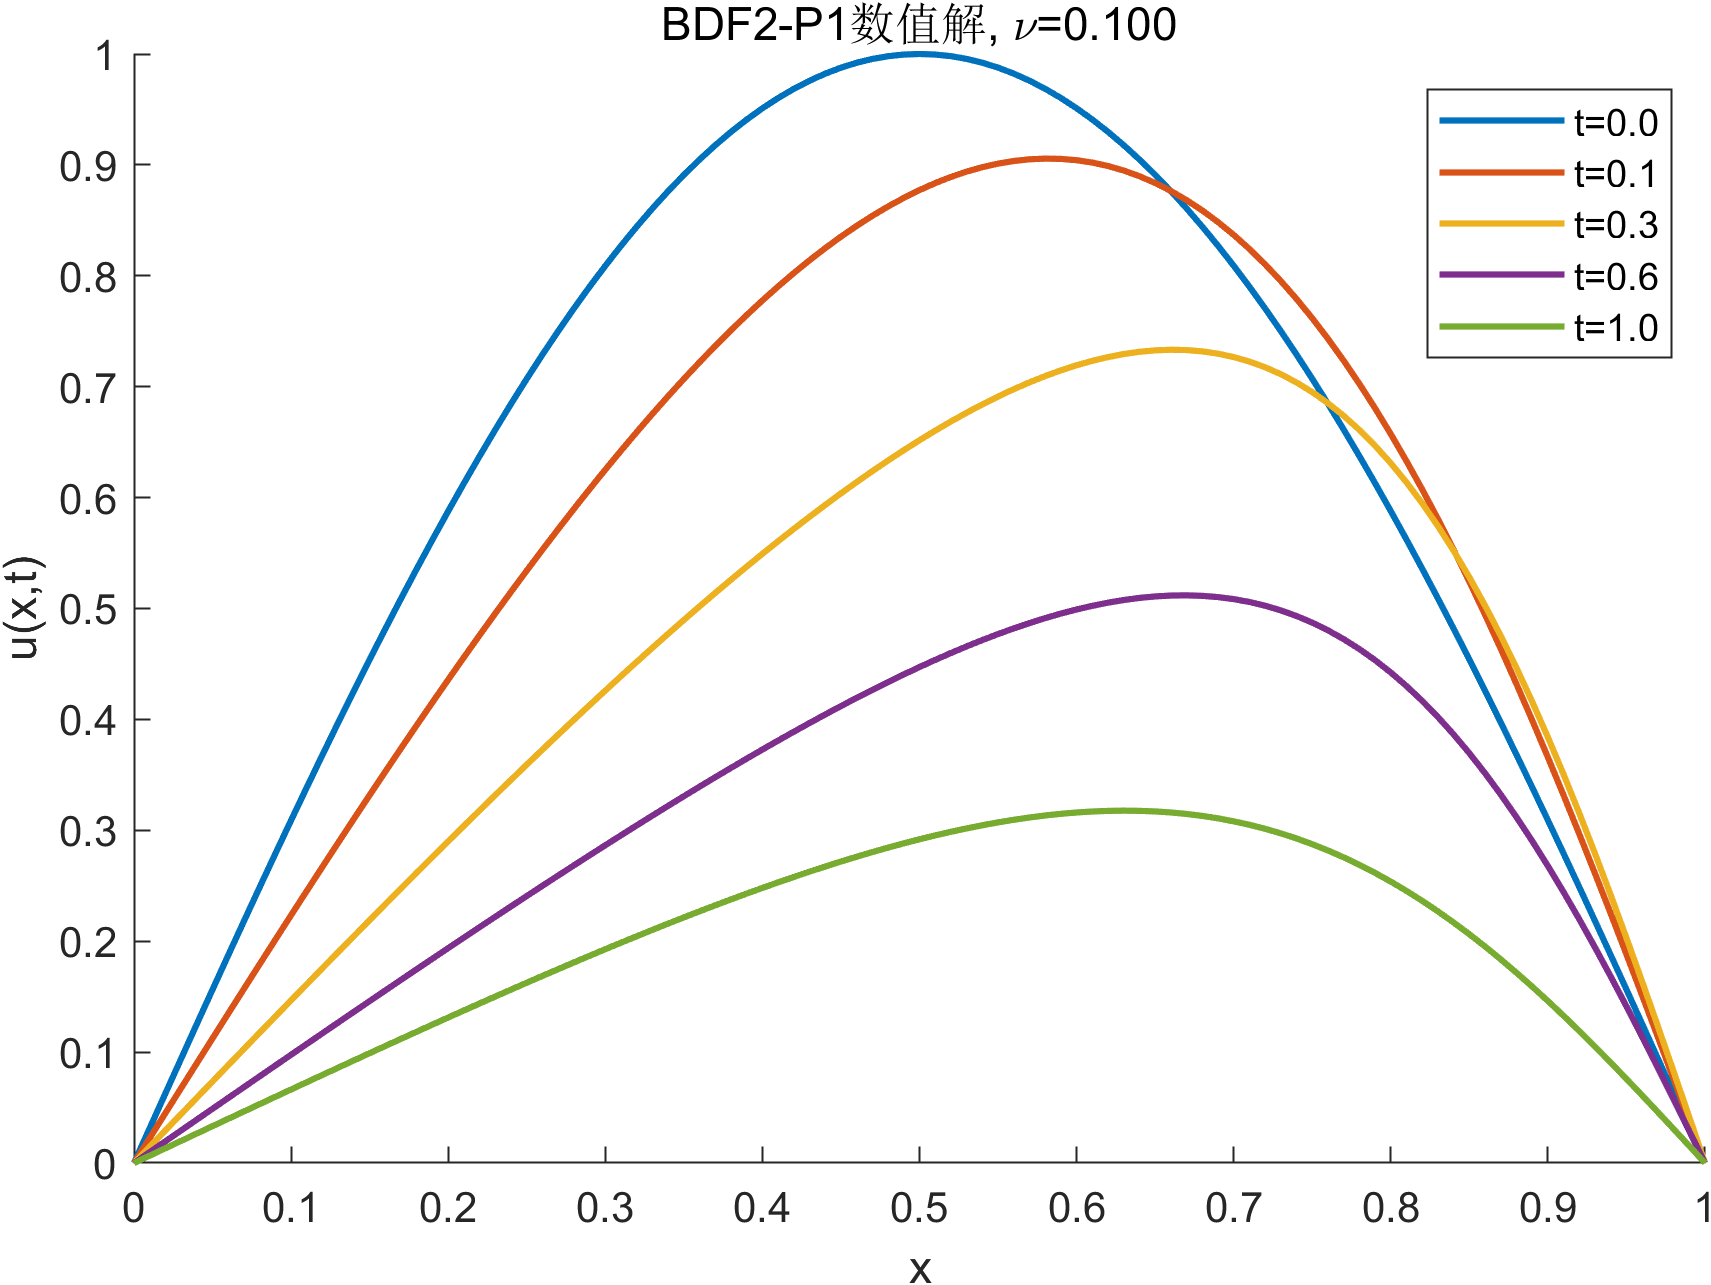
\includegraphics[width=\linewidth]{nonlinear.png}
				\footnotesize   图5：数值解在不同时刻的演化
			\end{column}
			\begin{column}{0.58\textwidth}
				\centering
				\small
				\textbf{在 $t=0.1$ 时刻的对比（$h=0.001$）}
				\vspace{0.05cm}
				\begin{tabular}{cccc}
					\toprule
					$x$ & 数值解 & 参考解析解 & $|u_h-u|$ \\
					\midrule
					0.1  & 0.22347 & 0.22345 & $2.0\times 10^{-5}$\\
					0.2  & 0.43584 & 0.43580 & $4.0\times 10^{-5}$\\
					0.3 & 0.62517 & 0.62512 & $5.0\times 10^{-5}$\\
					0.4 & 0.77776 & 0.77772  & $4.0\times 10^{-5}$\\
					0.5 & 0.87729 & 0.87728  & $1.0\times 10^{-5}$\\
					\bottomrule
				\end{tabular}
			\end{column}
		\end{columns}
		\vspace{2em}
		 图5展示初始正弦分布随时间右移且幅值衰减，符合耗散特性。
		
	\end{frame}
	\section{总结与展望}
\begin{frame}{总结与展望}
	\begin{enumerate}
		\item \textbf{总结}
		\begin{itemize}
			\setlength{\itemsep}{0.7em} 
				\item 空间 $P1$ 有限元 + 时间 BDF2 $\Rightarrow$ BDF2-P1 全离散
			\item $L^2$ 误差估计： $O(h^2+\tau^2)$，严格稳定性分析
			\item 数值实验：稳定，无非物理振荡，验证最优收敛
		\end{itemize}
	\vspace{0.3cm}
	 \item \textbf{展望}
	\begin{itemize}
		\setlength{\itemsep}{0.7em} 
		\item \textbf{精度：} 高阶元 + 高阶时间推进
		\item \textbf{推广：} 复杂非线性热传导
		\item \textbf{效率：} 自适应网格技术 / 并行算法
	\end{itemize}
		\end{enumerate}
\end{frame}
	\begin{frame}{致谢}
		\vfill
		\centering
		感谢各位老师、同学！\\[1cm]
		恳请各位专家批评指正！
		\vfill
	\end{frame}
\end{document}